\chapter{Question 5}
\section{Questions}
For $t$ in months, a population in thousands, is approximated by a continuous
function. \\
\[
P(t) =
\begin{cases}
  e^{kt} & 0 \leq t \leq 12 \\
  1000   & t > 12
\end{cases}
\]
\begin{enumerate}
  \item What is the initial value of the population?
  \item What must be the value of $k$?
  \item Describe in words how the population is changing.
\end{enumerate}

\section{Solutions}
\begin{enumerate}
  \item Initial value of the population at $t=0$:
  \begin{align}
    P(0) &= e^{k \cdot 0} \\
         &= e^0 \\
         &= 1
  \end{align}
  \item The value of $k$ needs to be determined to make $e^{k \cdot t}=1000$ at
  $t=12$.
  \begin{align}
    P(12) = 1000 &= e^{k \cdot 12} \\
    \ln(1000) &= k \cdot 12 \\
    \frac{\ln(1000)}{12} &= k \\
      &\approx 0.576...
  \end{align}
  We can substitute this back into the original equation:
  \[
  P(t) =
  \begin{cases}
    e^{ (\ln(1000)/12)\cdot t} & 0 \leq t \leq 12 \\
    1000   & t > 12
  \end{cases}
  \]
  \item Doubling time:
  \begin{align}
    2 &= e^{ (\ln(1000)/12)\cdot t} \\
    \ln(2) &= (\ln(1000)/12)\cdot t \\
    \frac{\ln(2)}{(\ln(1000)/12)} &= t \\
    \frac{12\ln(2)}{\ln(1000)} &= t \\
    t &\approx 1.2 \text{months}
  \end{align}

  The population is increasing exponentially (that is it doubles every 1.2
  months) until point $t$ at which point the population is constant (1000
  samples). A plot (figure \ref{fig:q5plot}) has been included which was
  generated by Mathematica from the following code:\\
  \texttt{
  Plot[Piecewise[{{E\^{}(Log[1000]t/12),t<=12},{1000,t>12}}],{t,0,14}]
  }
  \begin{figure}[!h]
    \centering
    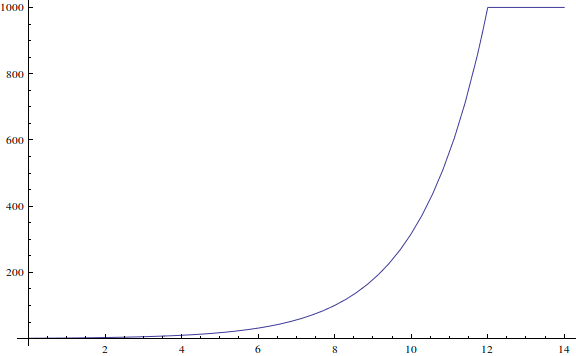
\includegraphics[width=\linewidth]{solutions/q5/q5plot.png}
  \caption{Plot of $e^{ (\ln(1000)/12)\cdot t}$.}
  \label{fig:q5plot}
  \end{figure}
\end{enumerate}\qedbitches
